%%%%%%%%%%%%%%%%%%%%%%%%%%%%%%%%%%%%%
%%%%%%%%%% Plantilla del Team para el proyecto final 
%%%%%%%%%%%%%%%%%%%%%%%%%%%%%%%%%%%%%
%%%%%%%%%% Nueva clase personalizada
\documentclass{staprojteamusb}
%%%%%%%%%% Nuevo estilo personalizado
\usepackage{staprojteamusbsty}

\addbibresource{referencias.bib}
%%%%%%%%%%%%%%%%%%%%%%%%%%%%%%%%%%%
%%%%%%%%%% Variables de Markdown
%%%%%%%%%%%%%%%%%%%%%%%%%%%%%%%%%%%
%%%%%%%%%% Encabezado 
\titulo{Análisis estadístico sobre una base de datos de beísbol.}

\autor{
		Miguel Cordero\\
	Universidad Simón Bolívar \\
	Caracas, Venezuela \\
	\texttt{\href{mailto:15-10326@usb.ve}{\nolinkurl{15-10326@usb.ve}}} \\
	 \And
		Eduardo Gavazut\\
	Universidad Simón Bolívar \\
	Caracas, Venezuela \\
	\texttt{\href{mailto:13-10524@usb.ve}{\nolinkurl{13-10524@usb.ve}}} \\
	 \And
		Luis Riera\\
	Universidad Simón Bolívar \\
	Caracas, Venezuela \\
	\texttt{\href{mailto:16-10976@usb.ve}{\nolinkurl{16-10976@usb.ve}}} \\
	}
\fecha{8 de abril de 2022}
\resumen{Este es un ejemplo de plantilla generado en RStudio para mostrar como se vería el proyecto final. Se realizarán una serie de análisis cuantitativos y cualitativos sobre una base de datos de beísbol. Se exponen los resultados y algunas conclusiones que se pueden extraer de los mismos. Cualquier error puede ser notificado para su corrección final. ESTO NO ES UN RESUMEN, se los estoy diciendo literal XD.}

\palabrasc{Proyecto, Estadistica, Rstudio, Beisbol}
%%%%%%%%%%%% Resto de las variables propias de R eso viene por defecto de R

%%%%%%%% Pandoc Estilo  de los codigos
\usepackage{color}
\usepackage{fancyvrb}
\newcommand{\VerbBar}{|}
\newcommand{\VERB}{\Verb[commandchars=\\\{\}]}
\DefineVerbatimEnvironment{Highlighting}{Verbatim}{commandchars=\\\{\}}
% Add ',fontsize=\small' for more characters per line
\usepackage{framed}
\definecolor{shadecolor}{RGB}{248,248,248}
\newenvironment{Shaded}{\begin{snugshade}}{\end{snugshade}}
\newcommand{\AlertTok}[1]{\textcolor[rgb]{0.94,0.16,0.16}{#1}}
\newcommand{\AnnotationTok}[1]{\textcolor[rgb]{0.56,0.35,0.01}{\textbf{\textit{#1}}}}
\newcommand{\AttributeTok}[1]{\textcolor[rgb]{0.77,0.63,0.00}{#1}}
\newcommand{\BaseNTok}[1]{\textcolor[rgb]{0.00,0.00,0.81}{#1}}
\newcommand{\BuiltInTok}[1]{#1}
\newcommand{\CharTok}[1]{\textcolor[rgb]{0.31,0.60,0.02}{#1}}
\newcommand{\CommentTok}[1]{\textcolor[rgb]{0.56,0.35,0.01}{\textit{#1}}}
\newcommand{\CommentVarTok}[1]{\textcolor[rgb]{0.56,0.35,0.01}{\textbf{\textit{#1}}}}
\newcommand{\ConstantTok}[1]{\textcolor[rgb]{0.00,0.00,0.00}{#1}}
\newcommand{\ControlFlowTok}[1]{\textcolor[rgb]{0.13,0.29,0.53}{\textbf{#1}}}
\newcommand{\DataTypeTok}[1]{\textcolor[rgb]{0.13,0.29,0.53}{#1}}
\newcommand{\DecValTok}[1]{\textcolor[rgb]{0.00,0.00,0.81}{#1}}
\newcommand{\DocumentationTok}[1]{\textcolor[rgb]{0.56,0.35,0.01}{\textbf{\textit{#1}}}}
\newcommand{\ErrorTok}[1]{\textcolor[rgb]{0.64,0.00,0.00}{\textbf{#1}}}
\newcommand{\ExtensionTok}[1]{#1}
\newcommand{\FloatTok}[1]{\textcolor[rgb]{0.00,0.00,0.81}{#1}}
\newcommand{\FunctionTok}[1]{\textcolor[rgb]{0.00,0.00,0.00}{#1}}
\newcommand{\ImportTok}[1]{#1}
\newcommand{\InformationTok}[1]{\textcolor[rgb]{0.56,0.35,0.01}{\textbf{\textit{#1}}}}
\newcommand{\KeywordTok}[1]{\textcolor[rgb]{0.13,0.29,0.53}{\textbf{#1}}}
\newcommand{\NormalTok}[1]{#1}
\newcommand{\OperatorTok}[1]{\textcolor[rgb]{0.81,0.36,0.00}{\textbf{#1}}}
\newcommand{\OtherTok}[1]{\textcolor[rgb]{0.56,0.35,0.01}{#1}}
\newcommand{\PreprocessorTok}[1]{\textcolor[rgb]{0.56,0.35,0.01}{\textit{#1}}}
\newcommand{\RegionMarkerTok}[1]{#1}
\newcommand{\SpecialCharTok}[1]{\textcolor[rgb]{0.00,0.00,0.00}{#1}}
\newcommand{\SpecialStringTok}[1]{\textcolor[rgb]{0.31,0.60,0.02}{#1}}
\newcommand{\StringTok}[1]{\textcolor[rgb]{0.31,0.60,0.02}{#1}}
\newcommand{\VariableTok}[1]{\textcolor[rgb]{0.00,0.00,0.00}{#1}}
\newcommand{\VerbatimStringTok}[1]{\textcolor[rgb]{0.31,0.60,0.02}{#1}}
\newcommand{\WarningTok}[1]{\textcolor[rgb]{0.56,0.35,0.01}{\textbf{\textit{#1}}}}

%%%%%%%%% Estilo de las listas sin salto de linea
\providecommand{\tightlist}{%
	\setlength{\itemsep}{0pt}\setlength{\parskip}{0pt}}

%%%%%%%%%%  Estilo de las tablas propias de R
\usepackage{longtable,booktabs,array}
\usepackage{calc} % Para la minipaginas y sus tamaños
%%%%%%%%%% Para las tablas y los parrafos \paragraph o \subparagraph
\usepackage{etoolbox}
\makeatletter
\patchcmd\longtable{\par}{\if@noskipsec\mbox{}\fi\par}{}{}
\makeatother
% Para los pie de pagina en tablas largas
\IfFileExists{footnotehyper.sty}{\usepackage{footnotehyper}}{\usepackage{footnote}}
\makesavenoteenv{longtable}

%%%%%%%%%%%% Si hay paquetes por incluir en header-include
\usepackage{booktabs}
\usepackage{longtable}
\usepackage{array}
\usepackage{multirow}
\usepackage{wrapfig}
\usepackage{float}
\usepackage{colortbl}
\usepackage{pdflscape}
\usepackage{tabu}
\usepackage{threeparttable}
\usepackage{threeparttablex}
\usepackage[normalem]{ulem}
\usepackage{makecell}
\usepackage{xcolor}
%%%%%%%%%%%%%%%%%%%%%%%%%%%%%%%%%%%%%%%%%%%%%%%%%%%%%%%%%
\begin{document}
	
	
	\maketitle
	
	%%%%%%%%%%%% Si hay cosas que incluir en include-before
		%%%%%%%%%%%%%%%%%%%%%%%%%%%%%%%%%%%%%%%%%%%%%%%%%%%%%%%%%
	
	%%%%%%%%%%%%% Inicio del documento
	
	\hypertarget{planteamiento-del-problema}{%
 \section{Planteamiento del problema}\label{planteamiento-del-problema}}

 Se desea realizar un análisis estadístico completo sobre una base de datos con información sobre el rendimiento de algunos jugadores de beisbol y en particular estudiar la relación (si la hay) de los hits al bate respecto a las carreras, dobles, triples, jonrones y ponches de los jugadores.

 \hypertarget{metododologuxeda}{%
 \subsection{Metododología}\label{metododologuxeda}}

 Para la realización de esta investigación se hará uso del sofware estadístico \texttt{R} en el entorno de desarrollo intergrado (IDE) \texttt{RStudio}. En este se iniciará por una descripción de los datos y variables almacenadas en el archivo fuente \emph{Baseball.xlsx}, tales como: mínimo, media, cuantiles y desviación estándar. Para la media de las variables se obtendrá un intervalo de confianza del \(95\%\). Como se desea estudiar la relación de la tasa de bateo respecto al resto de las variables, se buscará determinar la mejor distribución de probabilidad que se ajuste a esta variable. Finalmente, se estudiará la eficiencia del mejor modelo lineal de predicción que se ajuste a los datos y permita establecer si en efecto existe tal relación entre las variables y las implicaciones que tendría en las estrategias para futuros juegos de beisbol.

 \hypertarget{anuxe1lisis-de-los-datos}{%
 \section{Análisis de los datos}\label{anuxe1lisis-de-los-datos}}

 Para la realización de este proyecto se contó con una archivo de excel con la información de algunos jugadores de la Major League Beisbol o MLB, el cual se almacenó en una variable llamada \texttt{Baseball}:

 \hypertarget{realizar-un-anuxe1lisis-descriptivo-de-los-datos}{%
 \subsection{Realizar un análisis descriptivo de los datos}\label{realizar-un-anuxe1lisis-descriptivo-de-los-datos}}

 \hypertarget{quuxe9-clase-es-la-base-de-datos}{%
 \subsubsection{¿Qué clase es la base de datos?}\label{quuxe9-clase-es-la-base-de-datos}}

 Con el comando \texttt{class}, se pudo determinar el tipo de base de datos utilizada o lo que es equivalente, la clase de la variable \texttt{Baseball}.

 El resultado que se obtuvo indica que es del tipo \texttt{tbl\_df}, que es una subclase de la clase \texttt{data.frame}. \texttt{tbl\_df} cumple con tener propiedades diferentes por defecto y se suele referir a ellas como \texttt{tibble}. Es una clase eficiente para trabajar con bases de datos grandes y su visualización.

 \hypertarget{variables-en-la-base-de-datos}{%
 \subsubsection{Variables en la base de datos}\label{variables-en-la-base-de-datos}}

 Si se desea saber que tipo de variables están almacenadas en la base de datos, se puede utilizar el comando \texttt{str}. Esta función nos indica que se cuentan con \(6\) variables denominadas \texttt{X1,X2,X3,X4,X5,X6}, y distribuidas de tal manera que representan la columnas de la base de datos. Cada una de estas variables tienen \(45\) valores de tipo \texttt{double} o número decimal, que representan las \(45\) observaciones aleatorias (una por fila) realizadas a jugadores de la (MLB) .

 Cada variable representa la siguiente información:

 \begin{itemize}
 \tightlist
 \item
   \texttt{X1}: tasa de bateo, medido en hits por veces al bate.
 \item
   \texttt{X2}: tasa de carreras anotadas, medido en carreras anotadas por veces al bate.
 \item
   \texttt{X3}: tasa de dobles, medido en dobles por veces al bate.
 \item
   \texttt{X4}: tasa de triples, o los tripes por veces al bate.
 \item
   \texttt{X5}: tasa de jonrones, que son los jonrones por veces al bate.
 \item
   \texttt{X6}: tasa de ponches, medido como ponches por veces al bate.
 \end{itemize}

 \hypertarget{estaduxedsticos}{%
 \subsubsection{Estadísticos}\label{estaduxedsticos}}

 Para obtener los estadísticos de las seis (6) variables de esta base de datos, se inicia por guardar las \(45\) observaciones en un vector que represente a cada variable.

 Con los datos vectorizados se pueden aplicar las siguientes funciones: \texttt{mean} que permite obtener la media de los datos, \texttt{median} para obtener la mediana, \texttt{quantile} para retornar los cuantiles al \(0.25\%, 0.50\%\) y \(0.75\%\) de cada variable, \texttt{min} para el valor mínimo, \texttt{max} para el valor máximo, \texttt{var} para la varianza, \texttt{sd} que es para la desviación estándar, \texttt{IQR} es para el rango intercuartil y finalmente, el coeficiente de variación obtenido como \texttt{stad/media}.

 \begin{table}

 \caption{\label{tab:resumen}Resumen Estadístico de las variables}
 \centering
 \resizebox{\linewidth}{!}{
 \begin{tabular}[t]{l|c|c|c|c|c|c|c|c|c|c}
 \hline
   & Mínimo & 25\% & Media & Mediana (50\%) & 75\% & Máximo & RIC & Varianza & Desv. Estándar & Coef. Variación\\
 \hline
 X1 & 0.188 & 0.248 & 0.2805 & 0.290 & 0.308 & 0.367 & 0.060 & 0.0019 & 0.0440 & 0.1569\\
 \hline
 X2 & 0.064 & 0.119 & 0.1509 & 0.150 & 0.189 & 0.259 & 0.070 & 0.0018 & 0.0420 & 0.2784\\
 \hline
 X3 & 0.025 & 0.039 & 0.0464 & 0.045 & 0.053 & 0.068 & 0.014 & 0.0001 & 0.0105 & 0.2255\\
 \hline
 X4 & 0.001 & 0.007 & 0.0113 & 0.009 & 0.016 & 0.030 & 0.009 & 0.0000 & 0.0070 & 0.6165\\
 \hline
 X5 & 0.000 & 0.009 & 0.0243 & 0.013 & 0.039 & 0.085 & 0.030 & 0.0005 & 0.0223 & 0.9173\\
 \hline
 X6 & 0.000 & 0.062 & 0.1043 & 0.095 & 0.138 & 0.264 & 0.076 & 0.0040 & 0.0631 & 0.6044\\
 \hline
 \end{tabular}}
 \end{table}

 Los resultados pueden ser apreciados en la tabla \ref{tab:resumen}. De estos resultados hay varios puntos que podemos detacar. La varianza de los datos es muy baja indicativo que entre los datos hay pocos valores atípicos o muy dispersos, lo que se refleja en valores mas cercanos a la media. Misma interpretación se puede extender a la desviación estándar pues es la raíz cuadrada de la varianza.

 Una consecuencia de la baja varianza es que la media y la mediana son valores muy cercanos. Esto es particularmente útil al analizar el valor del \texttt{RIC}, que toma como medida central la mediana de los datos. Es decir, nos indica donde se encuentra el \(50\%\) de los datos, cuánto mas bajo es el valor del RIc menos dispersos estan los datos.

 Para un análisis mas detallado de como se relacionan las variables entre sí, podemos analizar los histogramas junto a los gráficos de cajas y bigotes.

 \vspace{10mm}

 \hypertarget{diagramas-e-histograma-de-los-datos-por-cada-variable}{%
 \subsubsection{Diagramas e histograma de los datos por cada variable}\label{diagramas-e-histograma-de-los-datos-por-cada-variable}}

 \begin{figure}
 \centering
 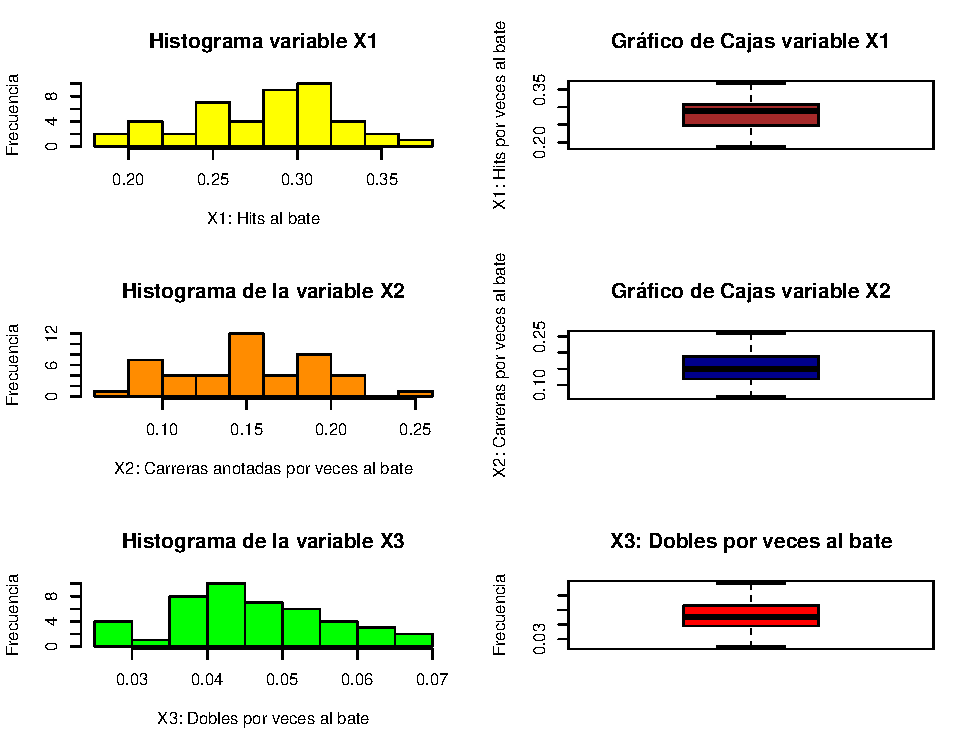
\includegraphics{C03322-InformeFinal-Cordero-Gavazut-Riera_files/figure-latex/boxplots-1.pdf}
 \caption{\label{fig:boxplots}Histograma y gráfico de cajas para las variables}
 \end{figure}

 \begin{figure}
 \centering
 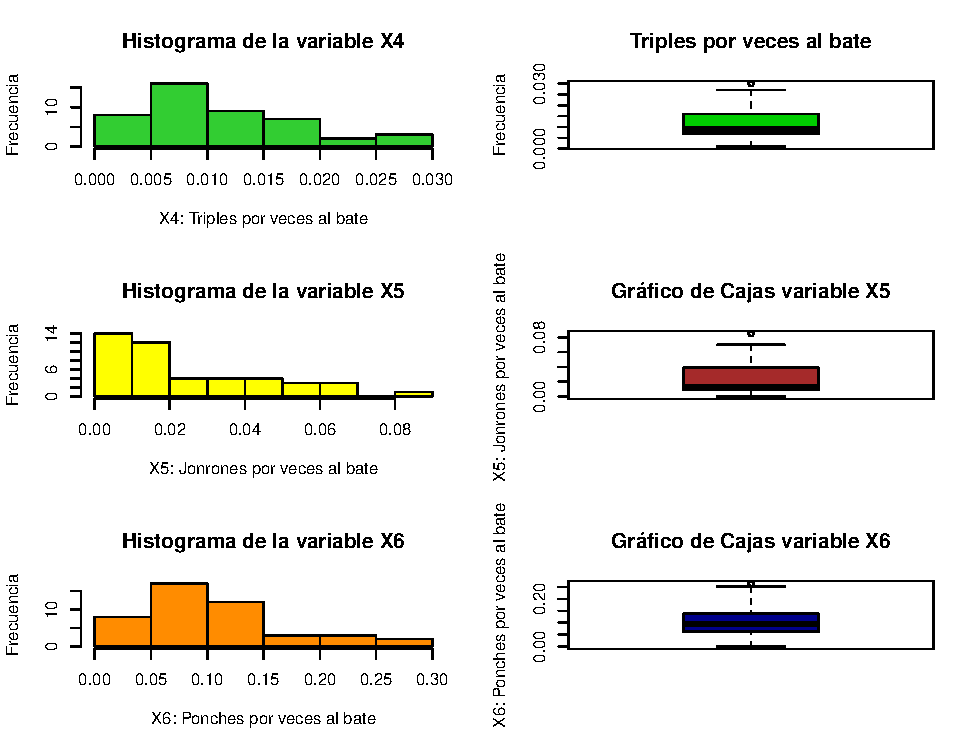
\includegraphics{C03322-InformeFinal-Cordero-Gavazut-Riera_files/figure-latex/boxplots2-1.pdf}
 \caption{\label{fig:boxplots2}Histograma y gráfico de cajas para las variables (continuación)}
 \end{figure}

 De la figura \ref{fig:boxplots} y la figura \ref{fig:boxplots2}, podemos establecer: para la variable \texttt{X1}, que los valores máximos de los datos se obtienen luego de la media, pero el mayor volumen de ellos se encuentra antes como bien se observa en el diagrama de caja que permite confirmar, además, la ausencia de datos atípicos. Para la variable \texttt{X2}, se puede comprobar que ver simetría de los datos que se infería de la tabla \ref{tab:resumem}, particularmente respecto al valor \(0.15\) que coincide a su vez con la media de los datos. El diagrama de caja permite confirmar la ausencia de los valores atípicos.

 Por su parte, para la variable \texttt{X3} y \texttt{X4}, Vemos que en general, ambos diagramas de caja son bastante parecidos, con la única diferencia siendo que el de triples está \(0.03\) puntos corrido hacia arriba y los datos desde el primer cuartil hasta la mediana están muchos más dispersos. Otra diferencia es que el diagrama de cajas para los triples no cuenta con datos atípicos, en cambio los dobles si, que corresponde a \(0.3\). Todo esto hace que el diagrama de los triples sea casi simétrico, y el de los dobles sea más chato entre el valor mínimo y la mediana, en comparación con lo que tenemos entre la mediana y el máximo valor.

 De la gráfica para la variable \texttt{X5} podemos ver como a medida que nos vamos acercando a \(1\) , la frecuencia de jonrones decae rapidamente, mientras que al incio es muy alta. De la gráfica para la variable \texttt{X6} podemos ver que la mayoria de los jugadores se ponchan menos de un \(15\%\) de las veces que estan al bate.

 \hypertarget{intervalo-de-confianza-para-la-media-de-las-variables}{%
 \subsection{Intervalo de confianza para la media de las variables}\label{intervalo-de-confianza-para-la-media-de-las-variables}}

 Con el uso de la función \texttt{t.test()} se puede encontrar el intervalo de confianza con una significancia de \(0.03\) o \(97\%\) de confianza para las variables estudiadas. Los resultados de aplicar esta función, se pueden visualizar en la tabla \ref{tab:intervals}.

 \begin{table}
 \caption{\label{tab:intervals}Intervalos del 97\% de confianza para las medias de las variables}
 \centering
 \resizebox{\linewidth}{!}{
 \begin{tabular}[t]{l|c|c|c}
 \hline
   & Limite inferior & Promedio & Limite Superior\\
 \hline
 Tasa de bateo & 0.2658 & 0.2805 & 0.2952\\
 \hline
 Carreras anotadas & 0.1368 & 0.1509 & 0.1649\\
 \hline
 Dobles & 0.0429 & 0.0464 & 0.0498\\
 \hline
 Triples & 0.0090 & 0.0113 & 0.0136\\
 \hline
 Jonrones & 0.0168 & 0.0243 & 0.0317\\
 \hline
 Ponches & 0.0833 & 0.1043 & 0.1254\\
 \hline
 \end{tabular}}
 \end{table}

 Vemos que para cada variable, los intervalos de confianza son

 \begin{enumerate}
   \item Tasa de bateo (hits/veces al bate): $(0.2657556, 0.2951778)$.
   \item Carreras anotadas (por veces al bate): $(0.1368441, 0.1649337)$.
   \item Dobles (por veces al bate): $(0.04286130, 0.04984981)$.
   \item Triples (por veces al bate): $(0.008962058, 0.013615720)$.
   \item Jonrones (por veces al bate): $(0.01682441, 0.03170892)$.
   \item Ponches (por veces al bate): $(0.08325165, 0.12541501)$.
 \end{enumerate}

 Ahora, para visualizar un poco mejor estos intervalos, pasemos a graficarlos con ayuda de la librería ggplot2:

 \begin{figure}
 \centering
 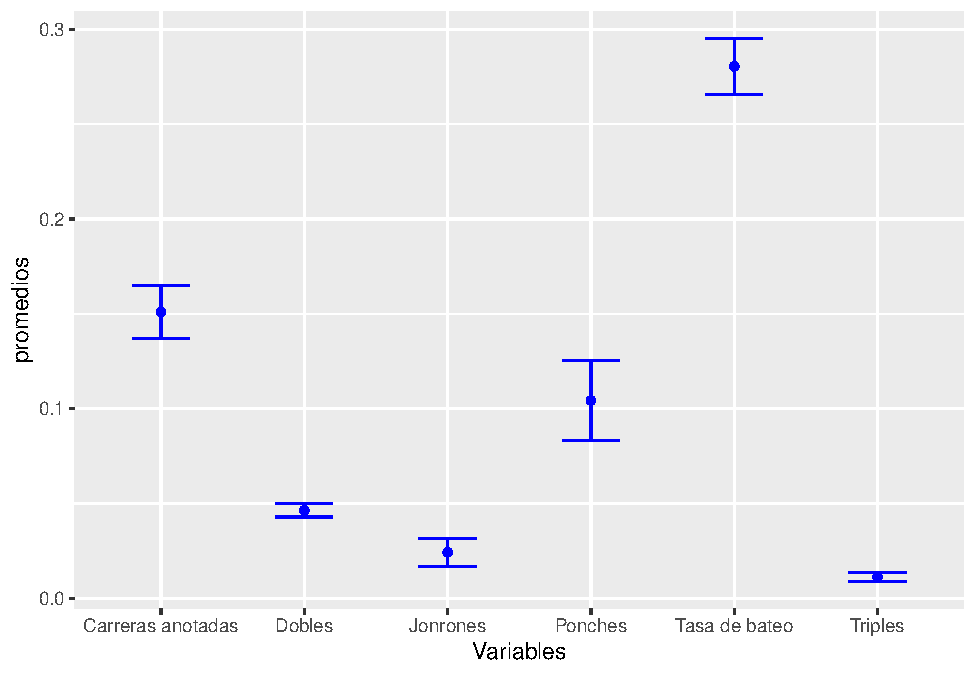
\includegraphics{C03322-InformeFinal-Cordero-Gavazut-Riera_files/figure-latex/unnamed-chunk-7-1.pdf}
 \caption{\label{fig:unnamed-chunk-7}Representación gráfica de los intervalos}
 \end{figure}

 Vemos que en general, los intervalos de confianza más estrechos son los de dobles y triples, lo que nos indica que en general, con una probabilidad del 97\%, podemos asegurar que los jugadores de la MLB tendrán un promedio de triples y dobles que puede ser estimado con bastante certeza, pero vemos que las carreras anotadas, los ponches y la tasa de bateo tienen un intervalo de confianza mucho más grande, por lo que no podemos asegurar que el promedio será estimado de forma tan certera.

 \hypertarget{promedio-de-bateo}{%
 \subsection{Promedio de bateo}\label{promedio-de-bateo}}

 Se desea probar con un nivel de significancia de \(\alpha=0.05\), que el promedio de bateo es inferior a \(0.300\).

 Como hipótesis nula \(H_{0}\), supongamos que la media de bateo, \(\overline{X1}\), es igual a \(0.3\). Y como hipótesis alternativa, \(H_{a}\), que el promedio de bateo es superior a \(0.3\), \(\overline{X1}>0.3\).

 Suponiendo que los datos presentan una distribución normal, podemos aplicar el comando \texttt{t.test}.

 Con este función, se obtuvo que el valor para el estadístico \(t\) es \(-23.811\), con \(44\) grados libertad. Como el \(p-valor\) es bastante alto, de hecho es igual \(0,9976\) (que representa un \(99.76\%\)), se cumple que \(\alpha=0.05<99.76\) y por lo tanto la hipótesis alternativa se rechaza, mas aún, se rechaza para todo nivel de significancia porque se necesita un valor para \(\alpha\) más alto que el \(p-valor\) para rechazar la hipótesis nula.

 Se afirma entonces, con total seguridad, que la tasa de bateo es inferior a \(0.300\).

 \hypertarget{comparaciuxf3n-entre-las-tasas-de-ponches-y-las-de-jonrones}{%
 \subsection{Comparación entre las tasas de ponches y las de jonrones}\label{comparaciuxf3n-entre-las-tasas-de-ponches-y-las-de-jonrones}}

 Queremos extraer la tasa de jonrones y de ponches al bate, estas variables corresponden a X5 y X6, respectivamente, entonces extraigámoslas de la base de datos

 Ahora, como no tenemos conocimiento acerca de las varianzas poblacionales, usaremos el test de Welch tal y como es explicado en Heumann, Schomaker (2017) para comparar las medias. En este caso, haremos una prueba de hipótesis, donde tomaremos como hipótesis

 \[
 H_0 : \mu_{\operatorname{jonrones}} - \mu_{\operatorname{ponches}} = 0 \text{ vs. } H_a : \mu_{\operatorname{jonrones}} - \mu_{\operatorname{ponches}} \neq 0
 \]

 es decir, queremos determinar si las tasas de jonrones y ponches son distintas. Ahora, usemos el \texttt{t.test()} para determinar cuál de estas hipótesis es aceptada:

\begin{verbatim}
## 
##  Welch Two Sample t-test
## 
## data:  jonrones and ponches
## t = -8.032, df = 54.799, p-value = 7.929e-11
## alternative hypothesis: true difference in means is not equal to 0
## 95 percent confidence interval:
##  -0.10004554 -0.06008779
## sample estimates:
##  mean of x  mean of y 
## 0.02426667 0.10433333
\end{verbatim}

 Vemos que el \(\operatorname{p-valor}\) es extremadamente pequeño, mucho más que el \(\alpha = 0.01\) que es razonable utilizar para nuestra prueba de hipótesis. Adicionalmente, vemos que en el intervalo de confianza no se incluye el cero. Otra cosa que podemos hacer es evaluar el estadístico de prueba con el comando \texttt{qt()} (vemos por lo anterior que \(dt = 55\) y \(\alpha = 0.05\)):

\begin{Shaded}
\begin{Highlighting}[]
\FunctionTok{qt}\NormalTok{(}\FloatTok{0.975}\NormalTok{, }\DecValTok{55}\NormalTok{)}
\end{Highlighting}
\end{Shaded}

\begin{verbatim}
## [1] 2.004045
\end{verbatim}

 Como \(t=-8\), vemos que el estadístico cae en la región de rechazo (porque es de cola doble).

 Para cualquiera de estos casos, podemos concluir que la hipótesis nula se rechaza, es decir que hay suficiente evidencia para creer que \(\mu_{\operatorname{jonrones}} - \mu_{\operatorname{ponches}} \neq 0\), además, como el intervalo de confianza es negativo, concluimos que \(\mu_{\operatorname{ponches}} > \mu_{\operatorname{jonrones}}\) con un nivel de confianza del \(95\%\).

 \hypertarget{gruxe1fico-de-dispersiuxf3n-y-matrix-de-correlaciuxf3n}{%
 \subsection{Gráfico de dispersión y matrix de correlación}\label{gruxe1fico-de-dispersiuxf3n-y-matrix-de-correlaciuxf3n}}

 \begin{figure}
 \centering
 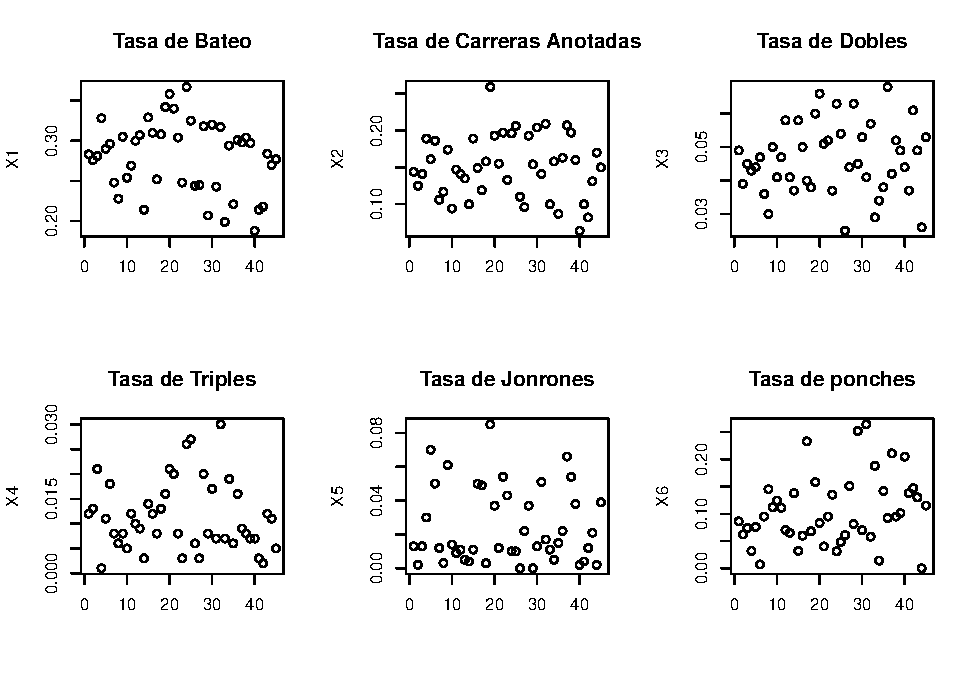
\includegraphics{C03322-InformeFinal-Cordero-Gavazut-Riera_files/figure-latex/unnamed-chunk-12-1.pdf}
 \caption{\label{fig:unnamed-chunk-12}Gráfico de Dispersión}
 \end{figure}

 \hypertarget{matriz-de-correlaciuxf3n}{%
 \subsection{Matriz de Correlación:}\label{matriz-de-correlaciuxf3n}}

 \begin{figure}
 \centering
 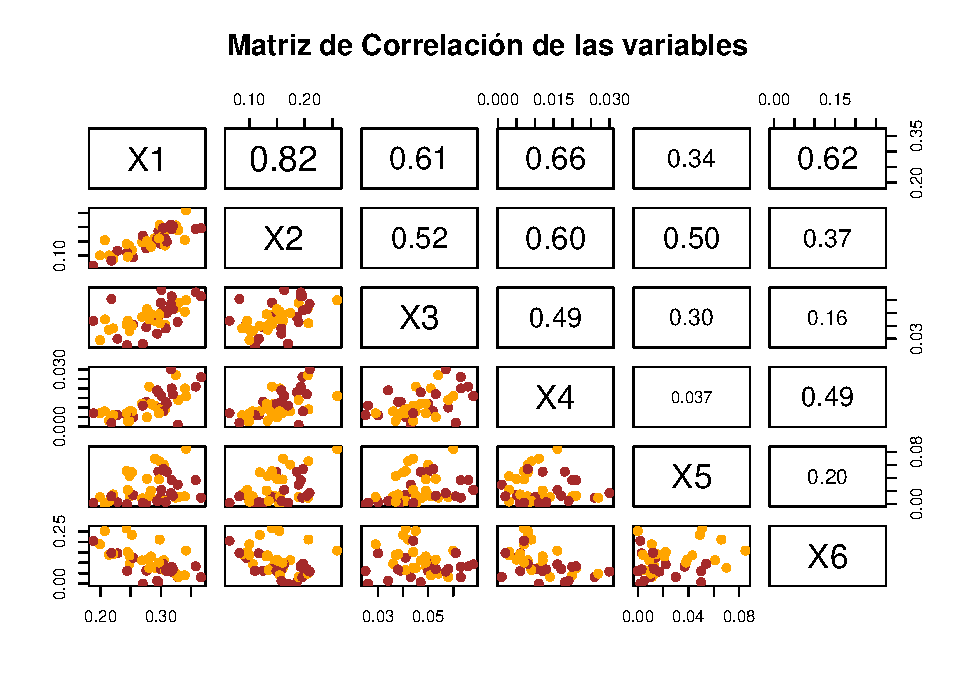
\includegraphics{C03322-InformeFinal-Cordero-Gavazut-Riera_files/figure-latex/unnamed-chunk-13-1.pdf}
 \caption{\label{fig:unnamed-chunk-13}Matrix de correlación}
 \end{figure}

 \newpage

 \hypertarget{referencias}{%
 \section{Referencias}\label{referencias}}

 Codigos utilizados en este informe:

\begin{Shaded}
\begin{Highlighting}[]
\CommentTok{\# Función para obtener un resumen estadístico completo de cada variable}
\NormalTok{estadisticos}\OtherTok{\textless{}{-}} \ControlFlowTok{function}\NormalTok{(variables)\{}
  \CommentTok{\# Inicializamos las variables}
\NormalTok{  k}\OtherTok{\textless{}{-}} \FunctionTok{length}\NormalTok{(variables)}
  \CommentTok{\# Minimo }
\NormalTok{  minimo }\OtherTok{\textless{}{-}} \FunctionTok{rep}\NormalTok{(}\DecValTok{0}\NormalTok{,k)}
  \CommentTok{\# Media}
\NormalTok{  media }\OtherTok{\textless{}{-}} \FunctionTok{rep}\NormalTok{(}\DecValTok{0}\NormalTok{,k)}
  \CommentTok{\# Mediana}
\NormalTok{  mediana}\OtherTok{\textless{}{-}} \FunctionTok{rep}\NormalTok{(}\DecValTok{0}\NormalTok{,k)}
  \CommentTok{\# Cuartile 1: 25\%}
\NormalTok{  q1 }\OtherTok{\textless{}{-}}\FunctionTok{rep}\NormalTok{(}\DecValTok{0}\NormalTok{,k)}
  \CommentTok{\# Cuartile 3: 75\%}
\NormalTok{  q3 }\OtherTok{\textless{}{-}} \FunctionTok{rep}\NormalTok{(}\DecValTok{0}\NormalTok{,k)}
  \CommentTok{\# Maximo }
\NormalTok{  maximo }\OtherTok{\textless{}{-}} \FunctionTok{rep}\NormalTok{(}\DecValTok{0}\NormalTok{,k)}
  \CommentTok{\# Rango Intercuartile }
\NormalTok{  ric }\OtherTok{\textless{}{-}} \FunctionTok{rep}\NormalTok{(}\DecValTok{0}\NormalTok{,k)}
  \CommentTok{\# Varianza }
\NormalTok{  varianza }\OtherTok{\textless{}{-}} \FunctionTok{rep}\NormalTok{(}\DecValTok{0}\NormalTok{,k)}
  \CommentTok{\# Desviación estándar}
\NormalTok{  stad }\OtherTok{\textless{}{-}}\FunctionTok{rep}\NormalTok{(}\DecValTok{0}\NormalTok{,k)}
  \CommentTok{\# Coeficiente de variación}
\NormalTok{  coef\_var }\OtherTok{\textless{}{-}}  \FunctionTok{rep}\NormalTok{(}\DecValTok{0}\NormalTok{,k)}
  
  \ControlFlowTok{for}\NormalTok{(i }\ControlFlowTok{in} \DecValTok{1}\SpecialCharTok{:}\NormalTok{k)\{}
    \CommentTok{\# Minimo }
\NormalTok{    minimo[i] }\OtherTok{\textless{}{-}} \FunctionTok{min}\NormalTok{(variables[,i])}
    \CommentTok{\# Media}
\NormalTok{    media[i] }\OtherTok{\textless{}{-}} \FunctionTok{mean}\NormalTok{(variables[,i])}
    \CommentTok{\# Mediana}
\NormalTok{    mediana[i]}\OtherTok{\textless{}{-}} \FunctionTok{median}\NormalTok{(variables[,i])}
    \CommentTok{\# Cuartile 1: 25\%}
\NormalTok{    q1[i] }\OtherTok{\textless{}{-}} \FunctionTok{quantile}\NormalTok{(variables[,i],}\FloatTok{0.25}\NormalTok{)}
    \CommentTok{\# Cuartile 3: 75\%}
\NormalTok{    q3[i] }\OtherTok{\textless{}{-}} \FunctionTok{quantile}\NormalTok{(variables[,i],}\FloatTok{0.75}\NormalTok{)}
    \CommentTok{\# Maximo }
\NormalTok{    maximo[i] }\OtherTok{\textless{}{-}} \FunctionTok{max}\NormalTok{(variables[,i])}
    \CommentTok{\# Rango Intercuartile }
\NormalTok{    ric[i] }\OtherTok{\textless{}{-}} \FunctionTok{IQR}\NormalTok{(variables[,i])}
    \CommentTok{\# Varianza }
\NormalTok{    varianza[i] }\OtherTok{\textless{}{-}} \FunctionTok{var}\NormalTok{(variables[,i])}
    \CommentTok{\# Desviación estándar}
\NormalTok{    stad[i] }\OtherTok{\textless{}{-}} \FunctionTok{sd}\NormalTok{(variables[,i])}
    \CommentTok{\# Coeficiente de variación}
\NormalTok{    coef\_var }\OtherTok{\textless{}{-}}\NormalTok{  stad}\SpecialCharTok{/}\NormalTok{media }
\NormalTok{  \}}
  
  \CommentTok{\# Unimos los valores obtenidos}
\NormalTok{  estadisticos }\OtherTok{\textless{}{-}} \FunctionTok{cbind}\NormalTok{(}\FunctionTok{round}\NormalTok{(minimo, }\AttributeTok{digits=}\DecValTok{4}\NormalTok{),}\FunctionTok{round}\NormalTok{(q1, }\AttributeTok{digits =} \DecValTok{4}\NormalTok{),}
                        \FunctionTok{round}\NormalTok{(media, }\AttributeTok{digits=}\DecValTok{4}\NormalTok{), }\FunctionTok{round}\NormalTok{(mediana,}\AttributeTok{digits=}\DecValTok{4}\NormalTok{),}
                        \FunctionTok{round}\NormalTok{(q3, }\AttributeTok{digits=}\DecValTok{4}\NormalTok{), }\FunctionTok{round}\NormalTok{(maximo, }\AttributeTok{digits=}\DecValTok{4}\NormalTok{),}
                        \FunctionTok{round}\NormalTok{(ric, }\AttributeTok{digits=}\DecValTok{4}\NormalTok{),}\FunctionTok{round}\NormalTok{(varianza, }\AttributeTok{digits=}\DecValTok{4}\NormalTok{), }
                        \FunctionTok{round}\NormalTok{(stad, }\AttributeTok{digits=}\DecValTok{4}\NormalTok{), }\FunctionTok{round}\NormalTok{(coef\_var, }\AttributeTok{digits=}\DecValTok{4}\NormalTok{))}
  \CommentTok{\# Definimos los nombres de las columnas y filas}
  \FunctionTok{rownames}\NormalTok{(estadisticos) }\OtherTok{\textless{}{-}} \FunctionTok{c}\NormalTok{(}\StringTok{"X1"}\NormalTok{, }\StringTok{"X2"}\NormalTok{, }\StringTok{"X3"}\NormalTok{, }\StringTok{"X4"}\NormalTok{, }\StringTok{"X5"}\NormalTok{, }\StringTok{"X6"}\NormalTok{) }
  \FunctionTok{colnames}\NormalTok{(estadisticos) }\OtherTok{\textless{}{-}} \FunctionTok{c}\NormalTok{(}\StringTok{"Minimo"}\NormalTok{, }\StringTok{"25\%"}\NormalTok{, }\StringTok{"Media"}\NormalTok{, }\StringTok{"Mediana / 50"}\NormalTok{ ,}
                              \StringTok{"75\%"}\NormalTok{, }\StringTok{"Máximo"}\NormalTok{, }\StringTok{"RIC"}\NormalTok{,}\StringTok{"Varianza"}\NormalTok{, }
                              \StringTok{"Desv. Estándar"}\NormalTok{,}\StringTok{"Coef. Variación"}\NormalTok{)}
  \CommentTok{\# Mostramos el arreglo}
  \FunctionTok{return}\NormalTok{(estadisticos)}
  
\NormalTok{\}}
\NormalTok{variables }\OtherTok{\textless{}{-}}\FunctionTok{as.data.frame}\NormalTok{(Baseball)}
\end{Highlighting}
\end{Shaded}

	
	%%%%%%%%%%%%% Fin del documento
	
	%%%%%%%%%%%% Inicio de la bibliografia
	\nocite{*}
	\printbibliography
	
	
	%%%%%%%%%%%%% Fin de la bibliografia
	
	%%%%%%%%%%%%%%%%% Si hay cosas que incluir en include-after
		%%%%%%%%%%%%%%%%%%%%%%%%%%%%%%%%%%%%%%%%%%%%%%%%%%%%%%%%%%%%
	
\end{document}
